\documentclass[a4paper,12pt,oneside,openany]{report}	

\usepackage{layout}
\setlength{\textwidth}{15.0 cm}
\setlength{\textheight}{25.0 cm}


\usepackage[english,brazil]{babel}
\usepackage{pagina}	% pagina-padrao
\usepackage{indentfirst}		% for indent
\usepackage[utf8x]{inputenc}
\usepackage{graphics,epsfig}
\usepackage{graphics}
\graphicspath{{./figuras/}}
\usepackage{pstricks,pst-node,pst-tree}
\usepackage{alltt}
%\usepackage{makeidx}
%\makeindex
\usepackage[figuresright]{rotating} % for saydways tables and figures
\usepackage{enumerate}			% for configuration of enumerate environment
\usepackage{amsmath}
\usepackage{amssymb}
\usepackage{multirow}

\setcounter{secnumdepth}{3}	% numeracao ate subsubsecao
\setcounter{tocdepth}{2}	% indice ate subsubsecao

\usepackage{longtable}


\begin{document}


\begin{center}
\textbf{UNIVERSIDADE FEDERAL DO RIO DE JANEIRO}
\vspace{-0.2cm}

\textbf{ESCOLA POLITÉCNICA}
\vspace{-0.2cm}

\textbf{DEPARTAMENTO DE ENGENHARIA ELETRÔNICA E DE COMPUTAÇÃO}
\vspace{0.8cm}

\underline{\textbf{PROPOSTA DE PROJETO DE GRADUAÇÃO}}

Aluno: Varlen Pavani Neto
\vspace{-0.2cm}

varlenneto@poli.ufrj.br

Orientador: Heraldo Luis Silveira de Almeida
\end{center}

\textbf{1. TÍTULO}

	Ferramenta para Tratamento de Informações Sensíveis em Bancos de Dados

\vspace{0.4cm}
\textbf{2. ÊNFASE}

Computação

\vspace{0.4cm}
\textbf{3. TEMA}

O tema do trabalho é o desenvolvimento de uma ferramenta que permita exportar informações dessensibilizadas e anonimizadas de um banco de dados.

\vspace{0.4cm}
\textbf{4. DELIMITAÇÃO}

O objeto de estudo do trabalho são processos de anonimização e garantia de privacidade em conjuntos de dados,
culminando na implementação de um software para realizar tais processos. No presente trabalho, as implementações destes processos serão estudados a partir de software livre.

\vspace{0.4cm}
\textbf{5. JUSTIFICATIVA}

A ubiquidade de dados pessoais produzidos pelo consumo de serviços digitais e o seu posterior entendimento como \textit{commodity} \cite{jmeyer} tem gerado uma crescente preocupação com a privacidade por parte das pessoas. 

Por muitas vezes a privacidade é vista como um direito fundamental\cite{solove}. Assim, a nível governamental esta preocupação foi transformada em legislação ao redor do mundo, como por exemplo o Regulamento Geral sobre a Proteção de Dados 2016/679 da União Europeia e a brasileira Lei Geral de Proteção de Dados Pessoais, Lei nº 13.709/2018.

Surge então nas instituições a necessidade de adequar processos e a maneira com que tratam seus dados à legislação vigente.

O presente projeto busca então complementar os modelos e técnicas, e revisar ferramentas existentes com o intuito de verificar seus pontos de melhoria e implementar um software de código aberto que auxilie as instituições a atingirem seus objetivos de conformidade com a lei, permitindo processar massas de dados sem perda de utilidade prática.

\vspace{0.4cm}
\textbf{6. OBJETIVO}

O objetivo geral deste trabalho é implementar um software livre que permita processar um banco de dados de modo a torná-lo dessensibilizado, podendo assim ser utilizado para apoiar atividades de desenvolvimento de sistemas sem a preocupação com vazamento de dados por parte de terceiros.

Sendo assim, os objetivos específicos a serem atingidos na implementação são: (1) O software deve remover informações que permitam associar indivíduos a um conjunto de dados; (2) O software deve substituir dados reais sensíveis por dados gerados a partir de estatísticas; (3) O software não deve alterar a estrutura do modelo de dados existente, somente o seu conteúdo.;

\vspace{0.4cm}
\textbf{7. METODOLOGIA}

Este trabalho inicialmente consiste num estudo das técnicas de anonimização de dados anteriormente aplicadas em dados médicos, que possuem necessidade de cuidados especiais de privacidade anterior a existência das leis de proteção de dados gerais, com o intuito de verificar como e quais técnicas podem ser utilizadas fora do contexto da informática para medicina. Para esta etapa inicial será feita uma revisão da literatura do assunto.

Em seguida, serão analisadas soluções de software livre existentes para verificar a implementação das técnicas exploradas anteriormente. Esta etapa contemplará softwares cuja licença seja aberta e estejam disponíveis no Github, tendo por objetivo caracterizar as funcionalidades existentes de modo a definir os requisitos do software a ser implementado, de maneira que este traga vantagens em relação as soluções existentes.

A partir da definição dos requisitos na etapa anterior, tem-se por inicio o desenvolvimento do código-fonte da nova solução. Esta solução será implementada utilizando a linguagem de programação Python, por se tratar de uma linguagem aberta e possuir suporte multiplataforma. Também será utilizada a biblioteca SQLAlchemy para implementar as atividades de acesso e manipulação dos bancos de dados, pois esta biblioteca fornece uma camada de abstração sobre diferentes implementações de APIs SQL\cite{sqlalch}, possibilitando que o projeto possa ser utilizado com diferentes implementações de bancos de dados SQL.

O alvo final deste trabalho é completar a implementação de um Minimum Viable Product com as funcionalidades determinadas anteriormente a ser validado sobre bases de dados públicas disponíveis na internet.

\vspace{0.4cm}
\textbf{8. MATERIAIS}
	
Serão utilizados software livres para estudo. Linguagem Python. Plataforma Github para controle de versão do código-fonte.

\vspace{0.4cm}
\textbf{9. CRONOGRAMA}

Apresentada graficamente conforme a Figura \ref{Fig:Cronograma}.

Fase 1: Estudo inicial sobre impacto socioeconômico causado pela visão de dados como commoditie

Fase 2: Análise bibliográfica de técnicas de privacidade e tópicos afins.

Fase 3: Estudo e levantamento das características de softwares de anonimização de código-aberto.

Fase 4: Implementação do código-fonte.

Fase 5: Testes com bases de dados públicas.

Fase 6: Revisão da Monografia

Fase 7: Elaboração da monografia


\begin{figure}
\begin{center}
\parbox[h]{14cm}
  {
  \begin{center}
  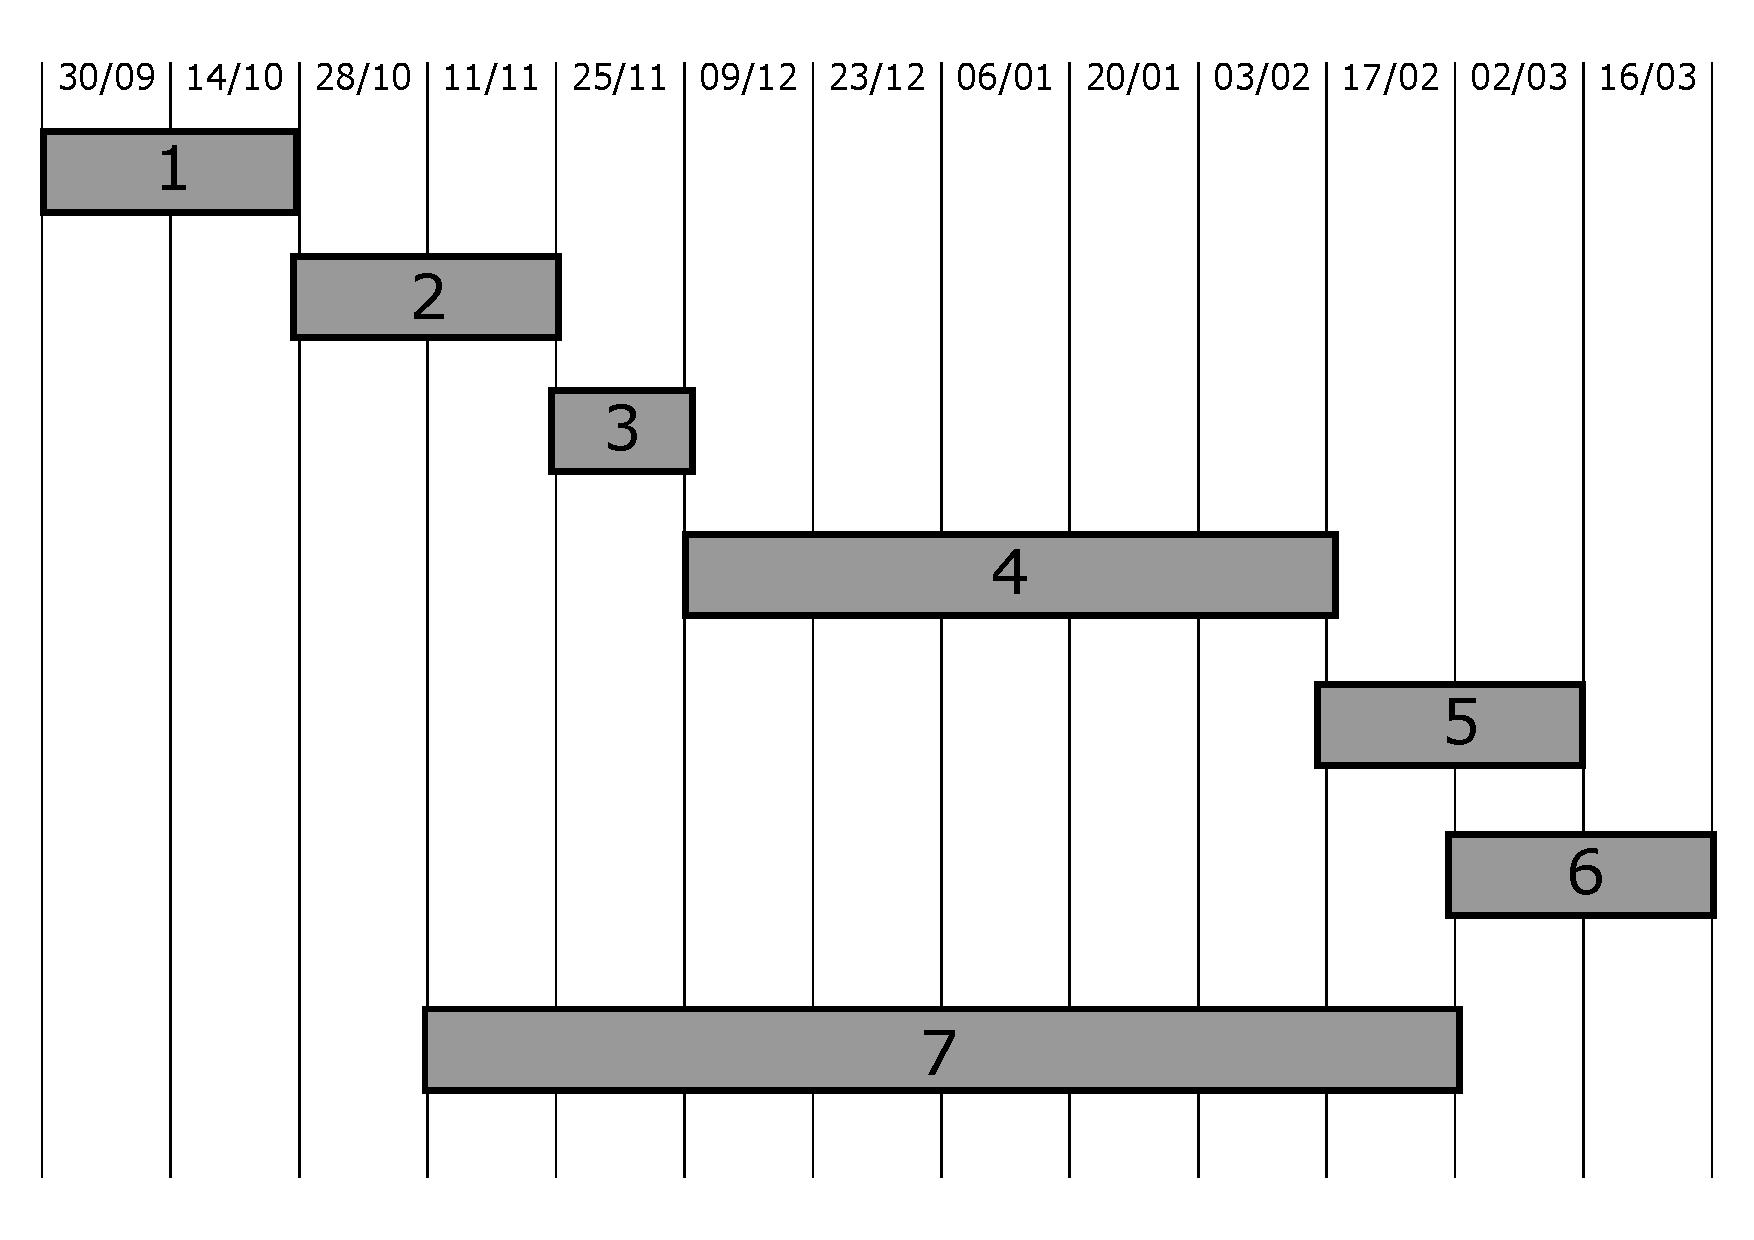
\includegraphics[scale=0.45]{Figuras/gantt.pdf}
  \caption[\small{\textit{Planejamento}}]{\label{Fig:Cronograma} \footnotesize{\textit{Planejamento}}}
  \end{center}
  }
\end{center}
\end{figure} 

\begin{thebibliography}{}

\bibitem{jmeyer} MEYER, Julie, "Personal data: time to argue about money, not privacy". Financial Times. https://www.ft.com/content/ba39f1a6-ea66-11e4-96ec-00144feab7de\#ixzz3YcJONvSE, 2013 (Acesso em 22 setembro 2019)

\bibitem{solove} SOLOVE, Daniel J. "Understanding privacy." Cambridge, MA: Harvard university press, 2008

\bibitem{sqlalch} "SQL Alchemy Features" - SQLAlchemy authors and contributors. https://www.sqlalchemy.org/features.html, 2019 (Acesso em 22 setembro 2019)

\end{thebibliography}

      \vspace{2cm}
      \noindent
Rio de Janeiro, 23 de setembro de 2019

      \vspace{0.5cm}
      \begin{flushright}
         \parbox{10cm}{
            \hrulefill

            \vspace{-.375cm}
            \centering{Varlen Pavani Neto - Aluno}

            \vspace{0.9cm}
            \hrulefill

            \vspace{-.375cm}
            \centering{Heraldo Luis Silveira de Almeida - Orientador}
 
            \vspace{0.9cm}
         }
      \end{flushright}
      \vfill
      
\end{document}
